% Scalar instruction entry source: tools/generate_scalar_instruction_catalog.py.
\subsection{\texttt{FCVT}}
\label{sec:scalar-fcvt}
\index{FCVT@\texttt{FCVT}}
\begin{sloppypar}\noindent\textbf{Purpose.} Converts SrcL between encoded floating-point formats using the default rounding mode and writes the result to RegDst.\end{sloppypar}\smallskip
\noindent\textbf{Syntax.}\par
\begin{lstlisting}[style=ptoscalarcode]
fcvt.{srcT2dstT} SrcL, ->RegDst
\end{lstlisting}
\noindent\textbf{Encoding.}\par
\noindent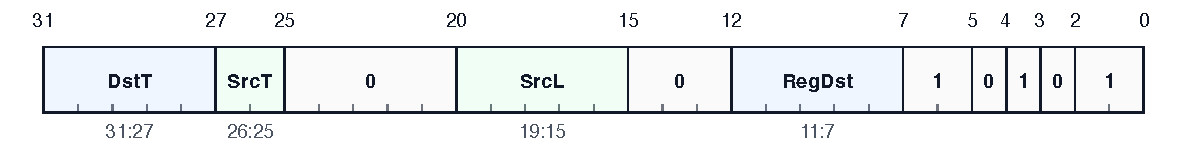
\includegraphics[width=\textwidth]{figs/encoding/scalar_instruction_entries/enc_fcvt.pdf}\par\smallskip
\begin{description}[leftmargin=0.18\linewidth,style=nextline]
\item[Format] \texttt{L32} \texttt{32-bit} scalar word.
\item[Pattern] \texttt{.......00000.....000.....1101011}.
\end{description}
\noindent\textbf{Classification.}\par
\begin{description}[leftmargin=0.18\linewidth,style=nextline]
\item[Category] Floating-Point and Conversion.
\item[Family] Format Convert.
\item[Execution class] \texttt{FSU}; uop\_kind=FSU.
\end{description}
\noindent\textbf{Operand fields.}\par
\begin{description}[leftmargin=0.18\linewidth,style=nextline]
\item[\texttt{DstType}] Bits \texttt{31:27 (5b)}. 5-bit destination format selector for conversion results. The assembly suffix \{srcT2dstT\} names the source and destination formats.
\item[\texttt{RegDst}] Bits \texttt{11:7 (5b)}. 5-bit scalar destination register that receives the floating-point, conversion, or FP-compare result encoded in scalar register storage; X0 discards the write.
\item[\texttt{SrcL}] Bits \texttt{19:15 (5b)}. 5-bit scalar source register holding the left or only floating-point/conversion operand; SrcType or the assembly suffix determines the interpreted format.
\item[\texttt{SrcType}] Bits \texttt{26:25 (2b)}. 2-bit source format selector for floating-point or conversion operands. The assembly suffix \{srcT2dstT\} names the source and destination formats.
\end{description}
\noindent\textbf{Operation.}\par
\begin{lstlisting}[style=ptoscalarcode]
value = Read(SrcL)
Write(RegDst, ConvertFormat(value, srcT, dstT, default_rounding))
\end{lstlisting}
\Needspace{0.08\textheight}
